% Inclusión de la figura histórica vectorial en escala de grises.
% El PDF y su fuente standalone se conservan literalmente como cubo_emrh_original.*.
\begin{figure}[htbp]
\centering
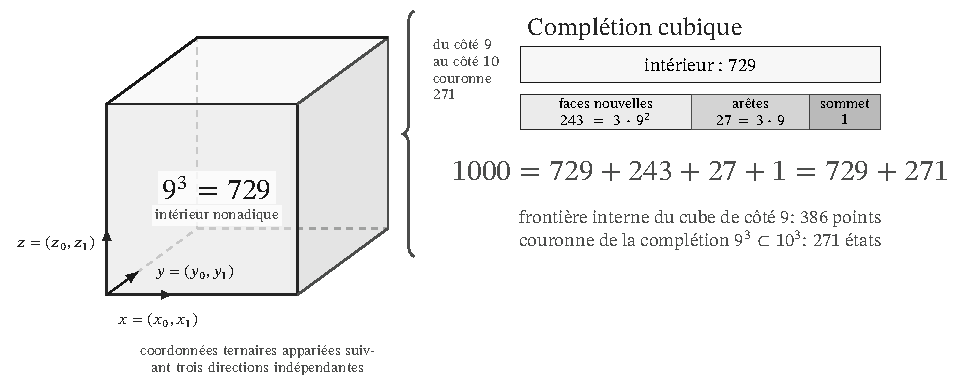
\includegraphics[width=\textwidth]{figures/cubo_emrh_original.pdf}
\caption{Représentation cubique de l'extension de neuf à dix classes par coordonnée. Les strates \(S_1,S_2,S_3\) placent les incidences ajoutées sur les faces, les arêtes et l'apex ; leurs cardinaux forment la couronne de \(271\) éléments. La frontière de \(386\) éléments appartient au cube initial. La perspective géométrique complète la partition de la figure ~\ref{fig:revision-emrh} ; les séparations graphiques ont une fonction schématique.}
\label{fig:completacion-cubo-recuperado}
\end{figure}
